Before migrating to Convolutional Neural Network(CNN) we tried many simple approaches for single-label image classification which we would use as a trained model for multi-label image classification. Though the accuracy of the approaches were not that good and also had many difficulties.

\section{Nearest Neighbor Classifier} 

The nearest neighbor classifier will take a test image, compare it to every single one of the training images, and predict the label of the closest training image. We compare the images pixel by pixel and add up all the differences. In other words, given two images and representing them as vectors $\big(I_{1},I_{2}\big)$ , a reasonable choice for comparing them might be the L1 distance:

\begin{equation}
 d_{1}(I_{1},I_{2}) =\sum_{p} \big(I_{1}^p-I_{2}^p\big)
\end{equation}

There are many other ways of computing distances between vectors. We can use the L2 distance, which has the geometric interpretation of computing the euclidean distance between two vectors.


\begin{equation}
 d_{1}(I_{1},I_{2}) = \sqrt{\sum_{p} \big(I_{1}^p-I_{2}^p\big)}
 \end{equation}
 
\paragraph{Accuracy}
\leavevmode \\
We got about $35\%$ using the NN Classifier.



\subsection{k - Nearest Neighbor Classifier}
Instead of finding the single closest image in the training set, we will find the top k closest images, and have them vote on the label of the test image. In particular, when k = 1, we recover the Nearest Neighbor classifier. The k-nearest neighbor classifier requires a setting for k. But what number works best? We have tried out many different values of k and experimented what k value works best.

\subsection{Cross-validation}
In cases where the size of the training data (and therefore also the validation data) is small, we can use a hyperparameter tuning called cross-validation. Instead of arbitrarily picking datapoints to be the validation set and rest training set, we can get a better and less noisy estimate of how well a certain value of k works by iterating over different validation sets and averaging the performance across these. For example, in 5-fold cross-validation, we would split the training data into 5 equal folds, use 4 of them for training, and 1 for validation.
\begin{figure}[h!]
  \centering
  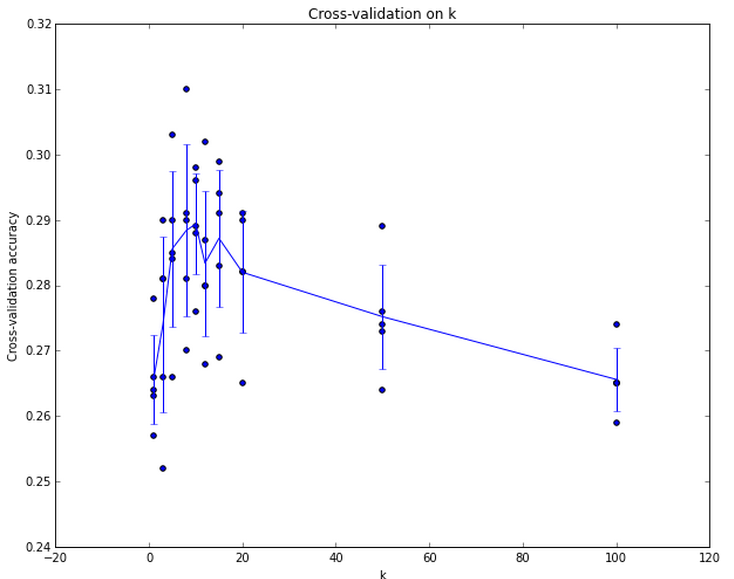
\includegraphics[width=1\textwidth]{knn.png}
  \label{fig2}
  \caption{Example of a 5-fold cross-validation run for the parameter k.}
\end{figure}

\subsubsection{Pros and cons of Nearest Neighbor Classifier}
\paragraph{Pros}
\leavevmode \\
1. It is very simple to implement and understand.
\leavevmode \\
2.  The classifier takes no time to train.
\paragraph{Cons}
\leavevmode \\
1. Accuracy rate is bad. 
\\
2. The classifier must remember all of the training data and store it for future comparisons.
\\
3. Using pixel differences to compare images is inadequate(Figure \ref{fig3})

\begin{figure}[h!]
  \centering
  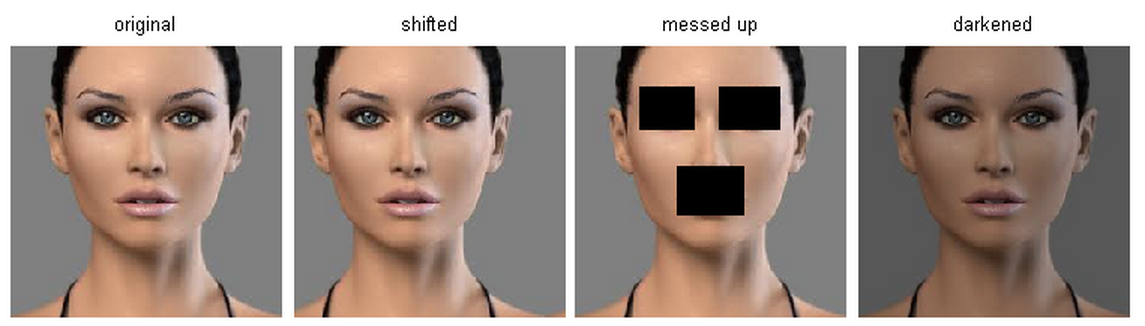
\includegraphics[width=1\textwidth]{consknn.png}
  \caption{Pixel-based distances on high-dimensional data (and images especially) can be very unintuitive. An original image (left) and three other images next to it that are all equally far away from it based on L2 pixel distance. Clearly, the pixel-wise distance does not correspond at all to perceptual or semantic similarity.}
  \label{fig3}
\end{figure}


\section{Linear Classification}
This approach will have two major components: a score function that maps the raw data to class scores, and a loss function that quantifies the agreement between the predicted scores and the ground truth labels. 


\paragraph{Score Function}
\leavevmode \\
For the score function we will use this linear mapping function:
\begin{equation}
 f(x_{i},W,b) = Wx_{i}+b
 \end{equation}
 
In the above equation, we are assuming that the image $x_{i}$ has all of its pixels flattened out to a single column vector of shape $[D*1]$. The matrix $W$ (of size $[K * D]$), and the vector b (of size $[K * 1]$) are the parameters of the function. In CIFAR-10 each image were of size $[32*32*3]$. Here  $x_{i}$ contains all pixels in the i-th image flattened into a single $[3072 * 1]$ column, W is $[10 * 3072]$ and b is $[10 * 1]$, so 3072 numbers come into the function (the raw pixel values) and 10 numbers come out (the class scores). The parameters in W are often called the weights, and b is called the bias vector because it influences the output scores.\hfill \break
An advantage of this approach is that the training data is used to learn the parameters W,b, but once the learning is complete we can discard the entire training set and only keep the learned parameters.
\paragraph{Cost Function}
\leavevmode \\
We will use a loss function called the Multiclass Support Vector Machine (SVM) loss. The SVM loss is set up so that the SVM wants the correct class for each image to a have a score higher than the incorrect classes by some fixed margin $\triangle$. So in each iteration if we achieve lower loss, then it is better. The Multiclass SVM loss for the i-th sample is :

\begin{equation}
 L_{i} =\sum_{i\not=j}max(0,f(x_{i},W)_{j}-f(x_{i},W)_{y_{i}}+\triangle)
 \end{equation}
 
\paragraph{Regularization}
There is an issue with loss function e.g. this set of W is not necessarily unique: there might be many similar W that correctly classify the examples. We can encode some preference for a certain set of weights W over others to remove this ambiguity. We can do so by extending the loss function with a regularization penalty $R(W)$.

\begin{equation}
R(W)=\sum_{k}\sum_{l}W_{k,l}^2 
\end{equation}

We told earlier that Multiclass Support Vector Machine loss is made up of two components: the data loss (which is the average loss $L_{i}$ over all examples) and the regularization loss. So the full Multiclass SVM loss becomes:

\begin{equation}
L= \dfrac{1}{N}\sum_{i}L_{i}+\lambda R(w)
\end{equation}


\section{Softmax Classifier}
In the Softmax classifier, the function mapping is as we used before on linear classifier. But we now interpret these scores as the unnormalized log probabilities for each class. Here we have a cross-entropy loss that has the form:
\begin{equation}
L_{i}=-log(\dfrac{e^{f_{y_{i}})}}{\sum_{j} e^{f_{j}}}
\end{equation}

\section{Optimization : Gradient Descent}
We need to improve our weight vector so that we can get lower loss. We need lower loss because loss function quantifies the agreement between the predicted scores and the ground truth labels. So obtaining lower loss means we are achieving better results. If we do a random search for best direction, then the computational cost will be higher. We can use gradient descent to compute the best direction along which we should change our weight vector. This direction will be related to the gradient of the loss function. This approach roughly corresponds to feeling the slope of the hill below our feet and stepping down the direction that feels steepest. The gradient is just a vector of slopes (more commonly referred to as derivatives) for each dimension in the input space.\hfill \break

By computing Gradient Descent, we are making an update of weight in the negative direction of the gradient since we wish our loss function to decrease, not increase.\hfill \break

Finally with the gradient descent we applied on SVM we get the decreasing loss in Figure 3.3. Also the accuracy was around $37\%$.
\begin{figure}[h!]
  \centering
  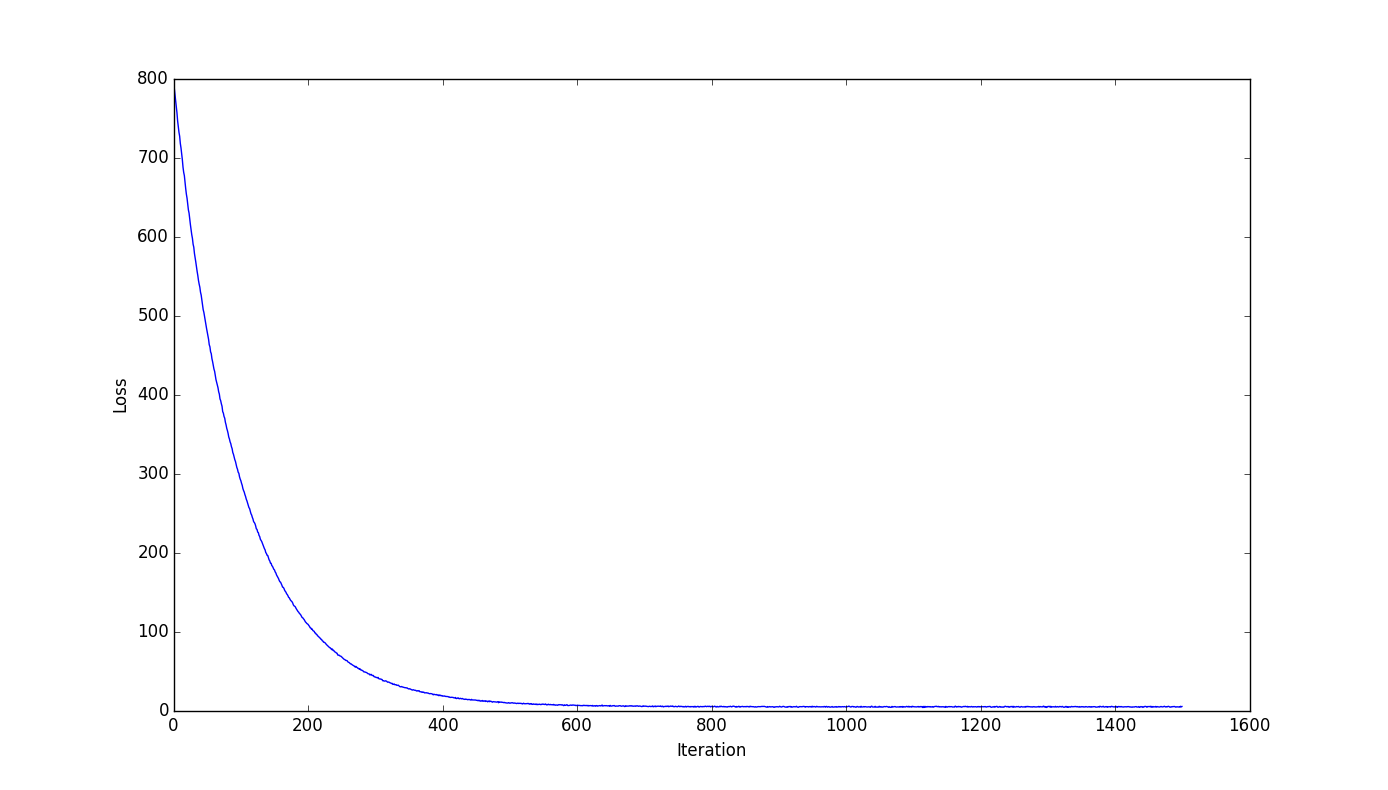
\includegraphics[width=1\textwidth]{svm.png}
  \caption{Decreasing loss as iteration increases}
  \label{fig4}
\end{figure}

\section{Neural Network in Object Detection}
Neural Networks are modeled as collections of neurons that are connected in an acyclic graph. In other words, the outputs of some neurons can become inputs to other neurons. For regular neural networks, the most common layer type is the fully-connected layer in which neurons between two adjacent layers are fully pairwise connected, but neurons within a single layer share no connections. 
\begin{figure}[h!]
  \centering
  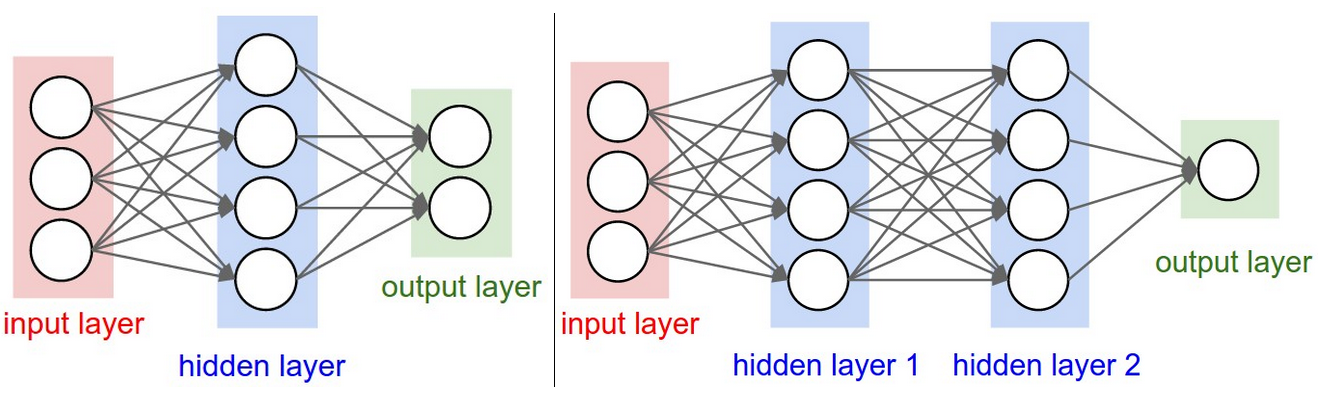
\includegraphics[width=0.7\textwidth]{neural.png}
  \caption{Left: A 2-layer Neural Network (one hidden layer of 4 neurons (or units) and one output layer with 2 neurons), and three inputs. Right: A 3-layer neural network with three inputs.}
  \label{fig5}
\end{figure}
\subsubsection{More Layers Better?}

If we increase the size and number of layers in a Neural Network, the capacity of the network increases. That is, the space of representable functions grows since the neurons can collaborate to express many different functions. In the Figure \ref{fig6} we see that higher hidden neuron means better representational power but it comes with a cost. The problem is overfitting.

\subsubsection{Overfitting}

Overfitting occurs when a model with high capacity fits the noise in the data instead of the underlying relationship. For example, the model with 20 hidden neurons fits all the training data but at the cost of segmenting the space into many disjoint red and green decision regions. A model which has been overfit will generally have poor performance on new data, as it can exaggerate minor fluctuations in the training set.

\begin{figure}[h!]
  \centering
  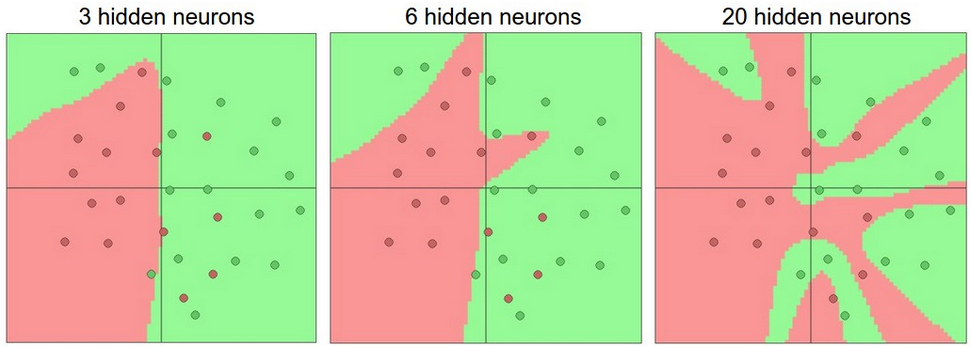
\includegraphics[width=1\textwidth]{neural2.png}
  \caption{Larger Neural Networks can represent more complicated functions. But more layers can also cause overfitting(example with 20 hidden neurons)}
  \label{fig6}
\end{figure}

\begin{figure}[h!]
  \centering
  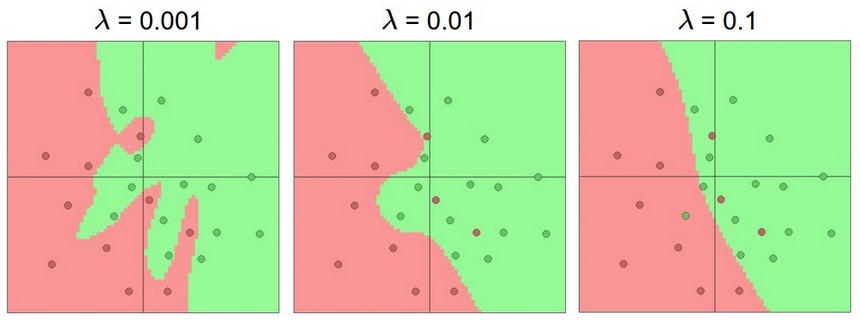
\includegraphics[width=1\textwidth]{neural3.png}
  \caption{The effects of regularization strength}
  \label{fig7}
\end{figure}

\subsubsection{How to control the overfitting?}
Regularization strength is the preferred way to control the overfitting of a neural network.

\begin{figure}[h!]
  \centering
  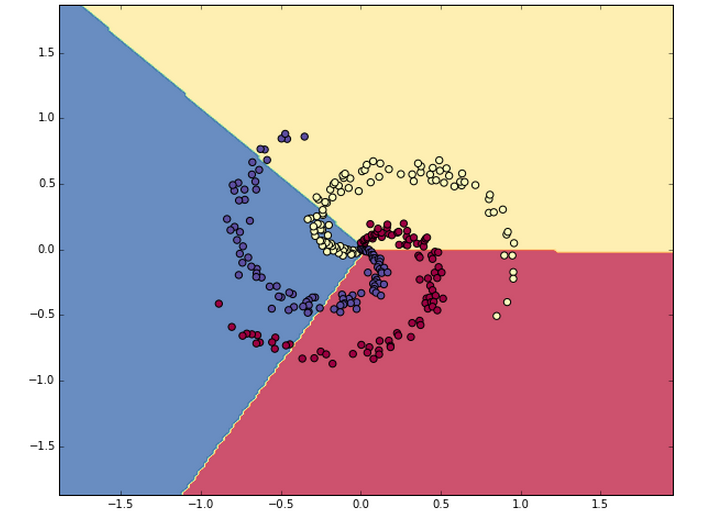
\includegraphics[width=.7\textwidth]{neural4.png}
  \caption{Linear classifier fails to learn the spiral dataset. Accuracy was around $49\%$}
  \label{fig8}
\end{figure}

\begin{figure}[h!]
  \centering
  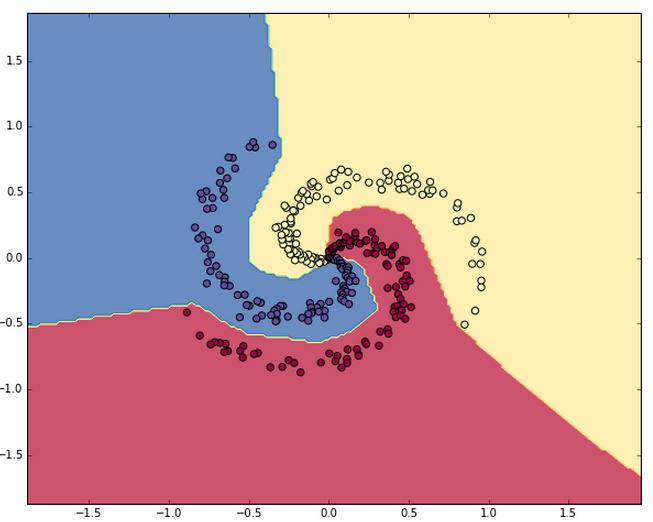
\includegraphics[width=.7\textwidth]{neural5.png}
  \caption{Neural Network classifier is significantly better achieving around $98\%$ accuracy}
  \label{fig9}
\end{figure}


\subsubsection{Linear Classifier vs. Neural Network}
If we implement a 2D dataset and tell any linear classifier to identify, it will fail to identify it correctly. Consider a spiral dataset containing 3 colors:yellow,blue and red. Now if we implement a linear classifier to identify each color in the 2D space we get a result similar to Figure \ref{fig8}.\hfill \break


If we use one additional hidden layer then we can get a lot better result.
\leavevmode
\\
Here we see that adding one additional layer helped us to attain bigger and better functionality.





